\documentclass[border=10pt]{standalone}
\usepackage[svgnames]{xcolor}
\usepackage{amsmath}
\usepackage{pgfplots}
\pgfplotsset{compat=newest}
\usepackage[sfdefault]{FiraSans}
\usepackage{FiraMono}
\renewcommand*\familydefault{\sfdefault}
\begin{document}
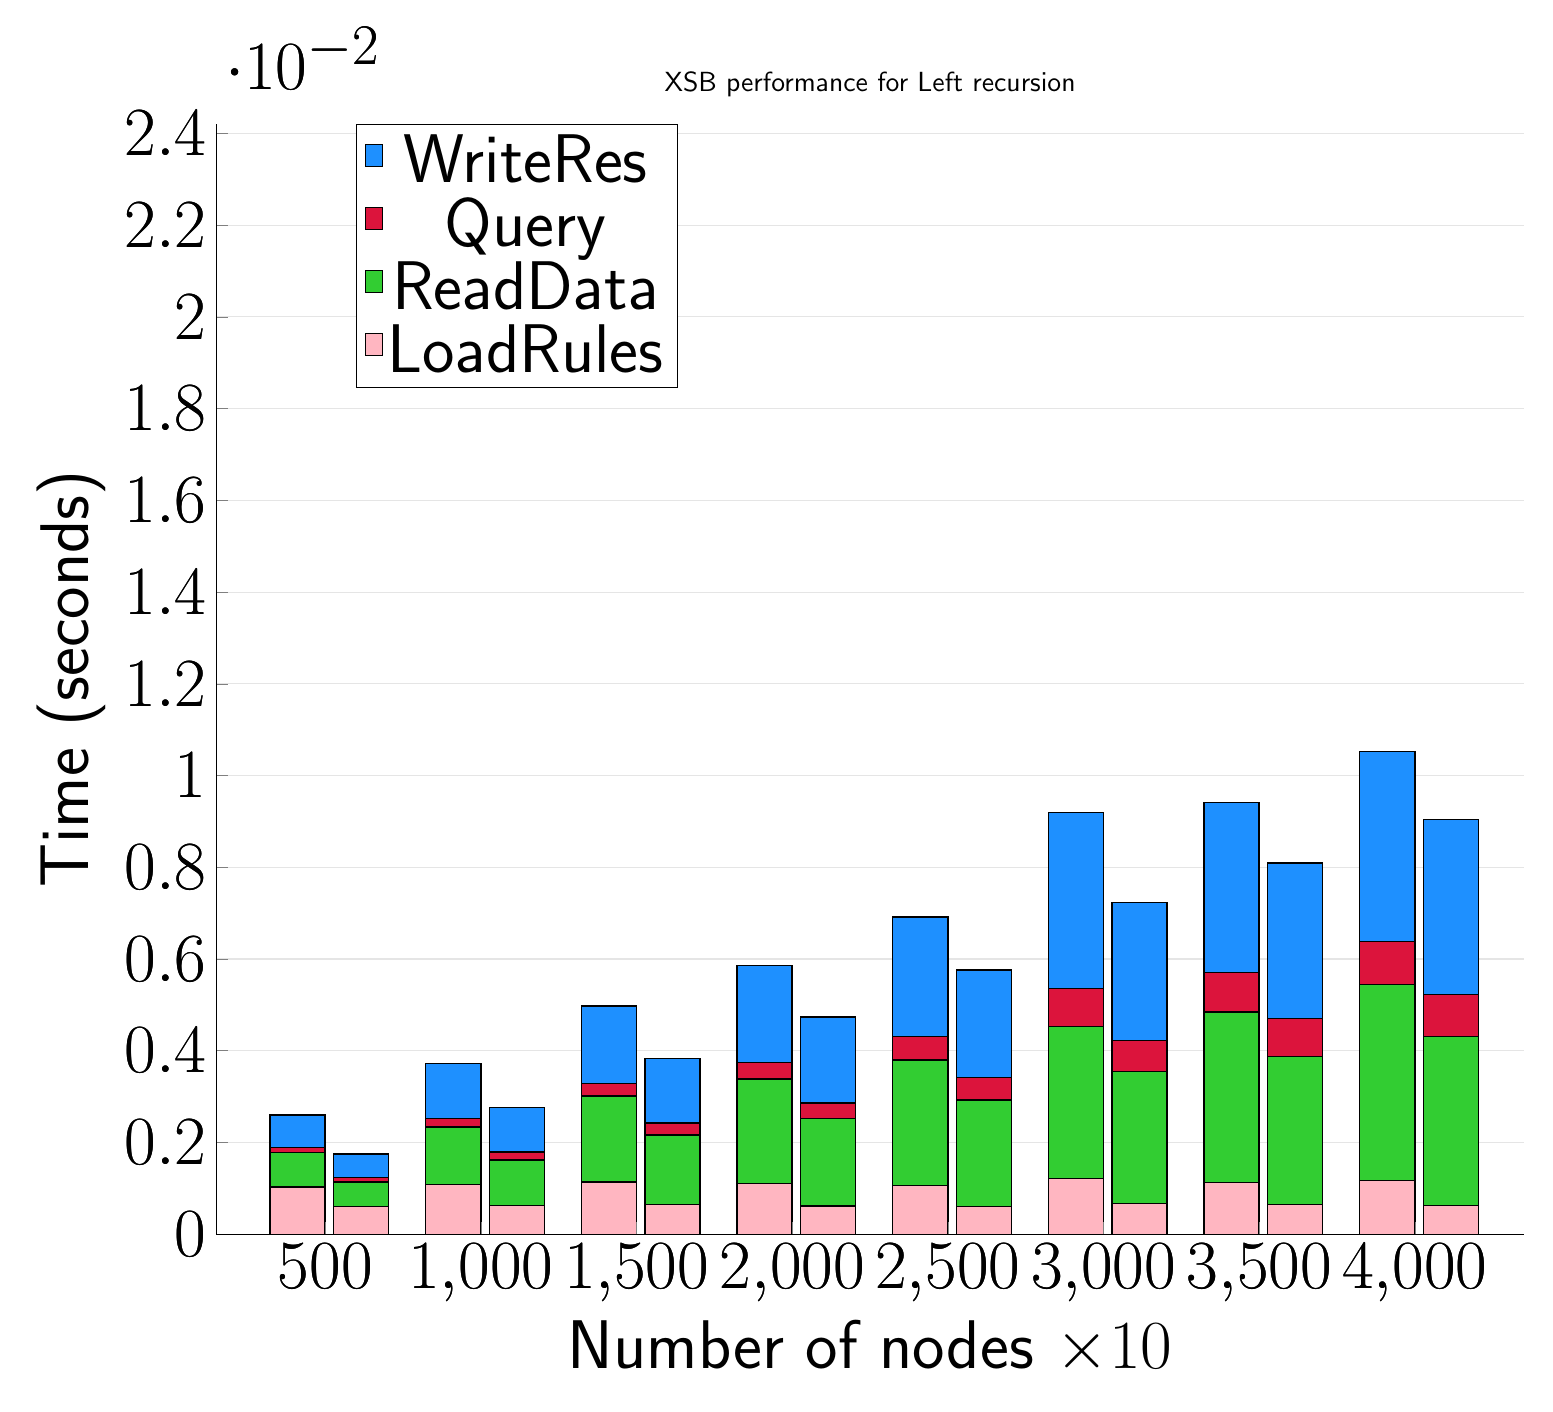
\begin{tikzpicture}
	\begin{axis}[
			ybar stacked,
			title={XSB performance for Left recursion},
			bar shift=-10pt,
			width=1.5\textwidth,
			bar width=0.7cm,
			ymajorgrids, tick align=inside,
			major grid style={draw=gray!20},
			xtick=data,
			ymin=0, ymax=0.024215764999389648,
			axis x line*=bottom,
			axis y line*=left,
			enlarge x limits=0.1,
			legend style={
					at={(0.23, 1)},
					anchor=north,
					legend columns=1,
					font=\Huge,
				},
			ylabel={Time (seconds)},
			xlabel={Number of nodes $\times 10$},
			label style={font=\Huge},
			tick label style={font=\Huge},
		]
		\addlegendimage{fill=DodgerBlue, draw=black, line width=0.2pt}
		\addlegendentry{WriteRes}
		\addlegendimage{fill=Crimson, draw=black, line width=0.2pt}
		\addlegendentry{Query}
		\addlegendimage{fill=LimeGreen, draw=black, line width=0.2pt}
		\addlegendentry{ReadData}
		\addlegendimage{fill=LightPink, draw=black, line width=0.2pt}
		\addlegendentry{LoadRules}
		\addplot +[fill=LightPink, draw=black, line width=0.5pt] coordinates {
				(500, 0.001032400131225584)
				(1000, 0.001087450981140137)
				(1500, 0.001138997077941894)
				(2000, 0.001100707054138183)
				(2500, 0.001061582565307617)
				(3000, 0.001211953163146974)
				(3500, 0.001125669479370118)
				(4000, 0.001176905632019043)
			};
		\addplot +[fill=LimeGreen, draw=black, line width=0.5pt] coordinates {
				(500, 0.0007557153701782226)
				(1000, 0.0012505769729614252)
				(1500, 0.001873946189880371)
				(2000, 0.0022851943969726548)
				(2500, 0.002733421325683592)
				(3000, 0.003312373161315918)
				(3500, 0.00372321605682373)
				(4000, 0.00426783561706543)
			};
		\addplot +[fill=Crimson, draw=black, line width=0.5pt] coordinates {
				(500, 9.856224060058596e-05)
				(1000, 0.0001820325851440429)
				(1500, 0.00027844905853271465)
				(2000, 0.00035591125488281254)
				(2500, 0.0005107641220092774)
				(3000, 0.0008358716964721683)
				(3500, 0.0008512496948242188)
				(4000, 0.0009425401687622071)
			};
		\addplot +[fill=DodgerBlue, draw=black, line width=0.5pt] coordinates {
				(500, 0.0007114410400390624)
				(1000, 0.0012039661407470704)
				(1500, 0.0016858816146850572)
				(2000, 0.00212085247039795)
				(2500, 0.0026119232177734355)
				(3000, 0.0038394451141357455)
				(3500, 0.0037188053131103514)
				(4000, 0.004138827323913575)
			};
	\end{axis}
	\begin{axis}[
			ybar stacked,
			bar shift=13pt,
			width=1.5\textwidth,
			bar width=0.7cm,
			ymajorgrids, tick align=inside,
			major grid style={draw=none},
			xtick=data,
			ymin=0, ymax=0.024215764999389648,
			axis x line*=none,
			axis y line*=none,
			enlarge x limits=0.1,
			label style={font=\Huge},
			tick label style={font=\Huge},
		]
		\addplot +[fill=LightPink, draw=black, line width=0.5pt] coordinates {
				(500, 0.0005996)
				(1000, 0.0006213000000000002)
				(1500, 0.0006450000000000001)
				(2000, 0.0006138999999999998)
				(2500, 0.0006094)
				(3000, 0.0006635999999999998)
				(3500, 0.0006411999999999998)
				(4000, 0.0006245000000000003)
			};
		\addplot +[fill=LimeGreen, draw=black, line width=0.5pt] coordinates {
				(500, 0.0005417999999999996)
				(1000, 0.0009953000000000004)
				(1500, 0.0015178999999999998)
				(2000, 0.0019105)
				(2500, 0.0023179000000000003)
				(3000, 0.0028798)
				(3500, 0.0032356999999999998)
				(4000, 0.0036857999999999995)
			};
		\addplot +[fill=Crimson, draw=black, line width=0.5pt] coordinates {
				(500, 8.940000000000041e-05)
				(1000, 0.0001718999999999993)
				(1500, 0.0002629000000000002)
				(2000, 0.0003371000000000002)
				(2500, 0.0004903000000000002)
				(3000, 0.0006750000000000003)
				(3500, 0.0008247)
				(4000, 0.0009096)
			};
		\addplot +[fill=DodgerBlue, draw=black, line width=0.5pt] coordinates {
				(500, 0.0005165999999999997)
				(1000, 0.0009742000000000006)
				(1500, 0.0014110999999999996)
				(2000, 0.0018723999999999998)
				(2500, 0.0023401)
				(3000, 0.0030097999999999995)
				(3500, 0.0033907)
				(4000, 0.003825)
			};
	\end{axis}
\end{tikzpicture}

\end{document}
